\subsection{Tridimenzionalna geometrija z GeoGebro}

GeoGebra 3D omogoča delo s tridimenzionalnimi objekti in njihovo vizualizacijo. V tem poglavju bomo raziskali osnovne funkcije GeoGebre 3D ter kako jih uporabiti za ustvarjanje in analizo tridimenzionalnih geometrijskih oblik.

Za delo v GeoGebri 3D moramo najprej preklopiti na 3D pogled. To storimo tako, da iz menija izberemo ``Perspectives'' in nato ``3D Graphics''. Prikaz ``3D Graphics'' vključuje tridimenzionalno koordinatno mrežo, ki nam omogoča ustvarjanje in manipulacijo 3D objektov, in tudi algebrsko okno, kjer lahko vidimo seznam vseh ustvarjenih objektov in njihovih lastnosti, podoben kot v 2D pogledu.

Točke v 3D prostoru ustvarimo z orodjem 
\includegraphics[width=0.0275\linewidth]{files/32px-Mode_point.svg-dc60e7c4e18f1e71b10806da1e7f4086.png}

 \textit{Point} (\textit{Točka}). Kliknemo na orodje in nato v 3D prostoru izberemo lokacijo, kjer želimo postaviti točko. Za to, moramo najprej določiti koordinate $x$ in $y$ v ravnini (sivi ravnini na 3D prikazu), nato pa določimo višino $z$ tako, da povlečemo točko navzgor ali navzdol. Ko ustvarimo točko, se njene koordinate prikažejo v algebrskem oknu. Alternativno lahko točko ustvarimo tudi z vnosom njenih koordinat v algebrsko okno, na primer \texttt{A = (2, 3, 4)}.

Podobno, za premikanje točk v 3D prostoru uporabimo orodje 
\includegraphics[width=0.0275\linewidth]{files/32px-Mode_move.svg-b420ab97c3d398837a03b0709d9d93f2.png}

 \textit{Move} (\textit{Premakni}). Nato lahko preklapljate med dvema načinoma s ponavljajočim klikom na točko, medtem ko je orodje aktivno: premikanje po ravnini (vzporedno v sivo ravnino) in premikanje navpično (v smeri osi $z$).

Najlažje način za učenje orodje je, da jih raziskujete.

\subsubsection{Točke in krogle}

Včasih je težko vse videti v 3D prostoru. Priporočamo, da eksperimentirate z različnimi pogledi in orodji za navigacijo v GeoGebri 3D. Vse najdete v 
\includegraphics[width=0.0275\linewidth]{files/32px-Stylingbar_icon-da79c17f9245fd7a577de157b0762fe4.png}

 \textit{Styling bar} (\textit{Vrstici za spremenite sloga pogleda}). Če želite ročno spremeniti pogled, uporabite orodje 
\includegraphics[width=0.0275\linewidth]{files/24px-Mode_rotateview-1ba2062ced630b55f4498b7eaa56a439.png}

 \textit{Rotate View} (\textit{Zasukaj pogled}) ali orodje 
\includegraphics[width=0.0275\linewidth]{files/32px-Mode_translatev-ebd873d304cfefb875a2544da650518a.png}

 \textit{Translate View} (\textit{Premakni pogled}).

\subsubsection{Premice in ravnine}

\subsubsection{Poliedri in drugi 3D objekti}

\subsubsection{Rotacijska ploskev}

Drugi način za prikaz rotacijske ploskve je z orodjem 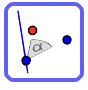
\includegraphics[width=0.0275\linewidth]{files/rotateAxis-2d3ed1b82acb9e1cff94634c58c97d2d.png}

 \textit{Rotate around Line} (\textit{Vrtenje okoli premice}).

\subsubsection{Funkcije z več spremenljivkami.}

\subsubsection{Vaje}\label{10_geogebra3D_vaje}

\begin{itemize}
\item Exercise~\ref{ex-spheres}: Ustvarite dve krogli v GeoGebri 3D in raziskujte njihovo presečišče.
\item Exercise~\ref{ex-distance}: Kako izmeriti razdaljo medo točkama v GeoGebri 3D?
\item Exercise~\ref{ex-cube}: Ustvarite kocko in ravnino v GeoGebri 3D ter poiščite njihovo presečišče.
\item Exercise~\ref{ex-polyhedra}: Ustvarite različne poliedre in 3D oblike v GeoGebri 3D.
\item Exercise~\ref{ex-rotational-surfaces}: Ustvarite rotacijske ploskve v GeoGebri 3D z vrtenjem daljic in krožnic okoli osi.
\item Exercise~\ref{ex-rotate-funkcije}: Ustvarite rotacijske ploskve z vrtenjem grafov funkcij okoli osi v GeoGebri 3D.
\item Exercise~\ref{ex-multivariable-functions}: Raziščujte funkcije z več spremenljivkami v GeoGebri 3D.
\end{itemize}